\chapter{Analysis and hardening of a FPGA Design with a MicroBlaze}

A SRAM-based FPGA is sensitive to SEUs, as explained in Chapter \ref{sec:background}. To better understand the effects of radiation on the FPGA, it is better to see a design as an abstraction of two layers. The two main layers are:

\begin{itemize}
    \item \textit{Application layer}: includes the logic and memory elements as described by the user.
    \item \textit{Configuration layer}: includes the logic and memory elements that are used to implement physically the user's design in the FPGA.
\end{itemize}

From the logical point of view, a particle causing a SEU can affects one of the two layers, producing different consequences:

\begin{itemize}
    \item SEUs in the Application Layer manifest as transient errors that could affect the stored data or the state of the user logic memory elements such as BRAMs or Flip-Flops. 
    \item SEUs affecting the Configuration Layer manifest as persistent errors, that could be reverted using a reconfiguration process. 
\end{itemize}

The first one are transients because they are in the user logic and are directly controlled by the user. Because of that, they may be detected or corrected, it depends on how the logic has been designed. The second one are persistent because they directly affects how the bottom hardware works: from the point of view of the user, it is like a real hardware fault that cannot be corrected. \bigskip

Persistent errors can have two main consequences:

\begin{itemize}
    \item They can change a routing element connection or can complete disconnect internal wires.
    \item They can change the behaviour of a LUT.
\end{itemize}

SEUs in the configuration layer are the most common type of errors in SRAM-based FPGAs because the application layer virtually uses less area than the configuration layer. A summary of the different causes of SEUs is presented in the following table:

\begin{table}[H]
\centering
    \begin{tabular}{|cc|cp{6.2cm}|}
        \hline
        \textbf{Layer} & & \textbf{Element} & \textbf{SEU Consequence} \\
        \hline
        \multirow{12}{*}{Configuration}
        & & Muxes & Wrong input selection, open net, wrongly driven or left open\\
        \cline{3-4}
        & Routing & PIP & Wrong connection or disconnection between nets\\
        \cline{3-4}
        & & Buffers & Output net wrongly driven or left open\\
        \cline{2-4}
        & & LUT & Wrong function inputs and outputs \\
        \cline{3-4}
        & Logic & Control Bits & Wrong function inputs and outputs\\
        \cline{3-4}
        & & Tie Offs & Wrong function initialization\\
        \hline
        \multirow{2}{*}{Application}
        & & RAM Blocks & Wrong application data\\
        \cline{3-4}
        & & CLB Flip-Flops & Wrong application data or state\\
        \hline
    \end{tabular}
\caption{SEU consequences in SRAM-based FPGAs \cite{10.1145/1046192.1046212}}
\label{tab:conseq_fpgas_seu}
\end{table}

The following analyzes are focused on SEUs affecting the configuration layer, as they are the most common type of errors in SRAM-based FPGAs. However, the proposed techniques allows designeers to detect and correct SEUs in the application layer, too.

\section{How SEUs affect the MicroBlaze?}

As anticipated in the previous sections, the object of interest of this thesis work is the analysis of the MicroBlaze behaviour when affected by SEUs and how those effects can be mitigated by constructing a series of ad-hoc hardening technique. \bigskip

First, in order to understand how the MicroBlaze reacts to SEUs affecting itself, a series of fault injection campaign must be executed. The idea is to start with a very minimal hardware design that includes a MicroBlaze and a set of minimal peripherals. Thanks to the Block Design tool, the preparation of the design is very simple and straightforward, and the result is shown in Figure \ref{fig:base_mb}:

\begin{figure}[H]
\centering
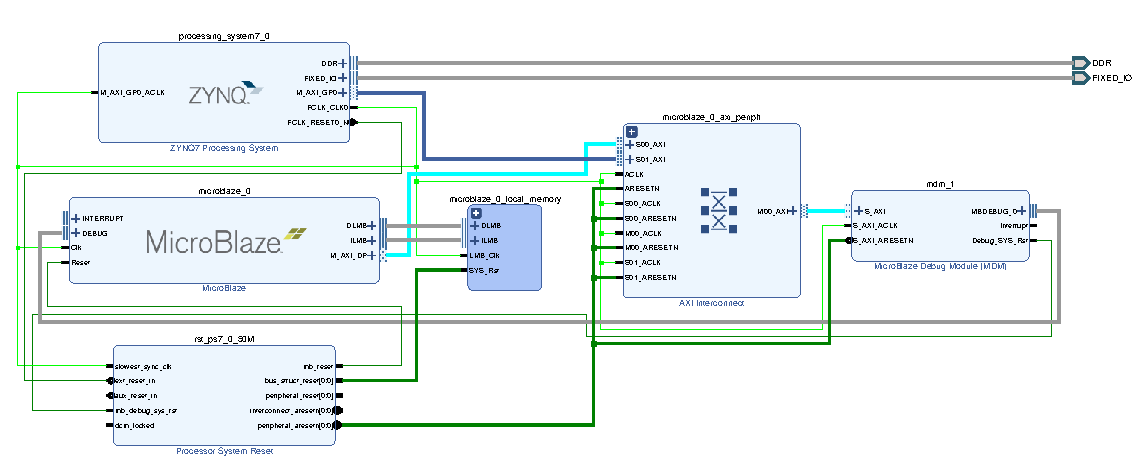
\includegraphics[width=1.0\linewidth]{images/chapter4/mb_base_design_edit.pdf}
\caption{Schematic of a basilar MicroBlaze design}
\label{fig:base_mb}
\end{figure}

In the schematic, the following blocks are present:
\begin{itemize}
    \item \textit{ZYNQ7 Processing System}: it represents the ZYNQ7020's Processing System (PS) from the point of view of the Programmable Logic (PL), as explained in Chapter \ref{sec:pynq}. It can offer a wide range of functionalities to the PL. For the moment, it is only used as a clock source and as a reset source. Via the ZYNQ7 PS block's configuration wizard, it is possible to configure a Phase-Locked Loop (PLL) in order to generate a clock for the PL with a specific frequency. For now, the PLL is configured to generate a clock for the PL with a frequency of 50 MHz, the same as the reference one given by the PYNQ-Z2 board.
    \item \textit{Processor System Reset}: is a soft IP that provides a mechanism to handle the reset conditions for a given system. The core handles numerous reset conditions at the input and generates appropriate resets at the output. For this simple design, the PSR is able to handle reset requests both from the PS and from the \textit{Debug Core}. It generates a active-high reset signal for the MicroBlaze core and for the Local Memory. Moreover, it generates a acthive-low reset signal for the AXI peripherals. 
    \item  \textit{MicroBlaze}: it represents the MicroBlaze instance under test. It has as inputs some debug signals from the Debug Core, the clock and the reset signal coming from the PSR. It offers as outputs the two memory buses for the Local Memory, one for the data memory (DLMB) and one for the instruction memory (ILMB). The last output is the AXI bus, which is used to access the peripherals through a \textit{AXI Interconnect}.
    \item \textit{Local Memory}: it is a sub-design (automatically generated by Vivado) that interfaces some BRAMs (a special kind of memory offered by the FPGA) with the Local Memory Bus (LMB). Block RAMs (or BRAMs) stands for Block Random Access Memory. Block RAMs are used for storing large amounts of data inside FPGAs.
    \item \textit{AXI Interconnect}: it is a sub-design (automatically generated by Vivado). As the name suggests, it is used to connect one or more AXI memory-mapped master devices to one or more memory-mapped slave devices.
    \item \textit{MicroBlaze Debug Module}: it is the Debug Core, and its main job is to enable JTAG-based software debugging of the MicroBlaze core. Moreover, it includes a configurable UART via an AXI interface. The UART's \textit{RX} and \textit{TX} signals are transmitted over the device JTAG port and can be accessed via the XSCT tool. With this setup, XSCT offers to designers the possibility to interact with the MicroBlaze core via a UART and to control the MicroBlaze core (status, registers, and software debug in general).
\end{itemize}

\begin{figure}[H]
\centering
\includegraphics[width=0.6\linewidth]{images/chapter4/hier.png}
\caption{Resulting hierarchy of the MicroBlaze design}
\label{fig:hier_mb}
\end{figure}

By looking at the schematic, there are two AXI masters connected to the AXI Interconnect. Hence, there are two different memory address spaces, and they are configured as follows:\bigskip

\begin{bytefield}{24}
    \begin{rightwordgroup}{/microblaze\_0}
        \memsection{0x4140\_0fff}{0x4140\_0000}{3}{4 KB MDM UART}\\
        \memsection{0x413f\_ffff}{0x0001\_0000}{3}{-- reserved --}\\
        \memsection{0x0000\_ffff}{0x0000\_0000}{6}{64 KB DLMB}
    \end{rightwordgroup}\\\\
    \begin{rightwordgroup}{/processing\_system7\_0}     
        \memsection{0x4140\_0fff}{0x4140\_0000}{3}{4 KB MDM UART}
    \end{rightwordgroup}
\end{bytefield}\bigskip

Finally, the design definition is ready and it can be synthesized and implemented. Because the aim of this design is to be analyzed by injecting faults, the MicroBlaze has been constrained to be placed in a specific portion of the FPGA, as explained in Chapter \ref{sec:fitollo}. This is possible with Vivado by defining a PBLOCK. \bigskip

A PBLOCK is a collection of cells, grouped in one rectangular area or region that specify the device resources contained by the PBLOCK. PBLOCKs are used during floorplanning. A design floorplan is broadly defined as a set of physical constraints used to control how the logic is placed into the FPGA. A good floorplan can help reduce routing congestion and improve the quality of timing results. On the other hand, a bad floorplan can reduce performances as well as unmet constraints if the required placement is unfeasible. \bigskip

As an example, the above design is implemented with the following constraints:

\begin{lstlisting}[style=tcl]
create_pblock pblock_1
add_cells_to_pblock [get_pblocks pblock_1] [
    get_cells -quiet [
        list design_1_i/microblaze_0
    ]
]

resize_pblock [get_pblocks pblock_1] -add {
    SLICE_X54Y102:SLICE_X67Y148
}

set_property IS_SOFT 0 [get_pblocks pblock_1]
\end{lstlisting}

In the above constraints, a PBLOCK called \textit{pblock\_1} is first defined. Than all the cells belonging to the Microblaze instance (\textit{design\_1\_i/microblaze\_0}) are added to the PBLOCK, and finally the PBLOCK is resized. The resize operation is used to define the physical resources that are included in the PBLOCK. As final operation, the PBLOCK is marked as a \textit{not soft} PBLOCK, which means that each MicroBlaze cell must be placed in that specific PBLOCK, and so it is a hard constraint.\bigskip

Once the constraints are ready, the design can be synthesized and implemented. The resulting floorplan is shown in the following figure:

\begin{figure}[H]
\centering
\includegraphics[width=0.7\linewidth]{images/chapter4/impl.png}
\caption{Resulting floorplan of the MicroBlaze design, with the PBLOCK on the top side. Microblaze cells are highlighted in red}
\end{figure}

Finally, it is possible to launch the fault injection tool by providing the bitstream with no CRC and a .elf file to be executed by the MicroBlaze at each run. The resulting fault injection campaign is shown in the following:

\begin{table}[H]
\small
\centering
\begin{tabular}{ l|rr }
    \hline
    \multicolumn{3}{|c|}{\textbf{Functional Analysis}} \\
    \hline
    &\textit{Total}&\textit{Percentage} \\
    \cline{2-3}
    Correct results & 9618 & 77.94 \%\\
    Faulty results (SDE) & 131 & 1.06 \%\\
    MicroBlaze halted & 2359 & 19.12 \%\\
    Raised exceptions & 233 & 1.89 \%\\
    \hline
    Total injected bitflips & 12341 & 100.00 \%\\
    \\
    \hline
    \multicolumn{3}{|c|}{\textbf{Exceptions}}\\
    \hline
    &\textit{Total}&\textit{Percentage} \\
    \cline{2-3}
    \small
    \texttt{XEXC\_ID\_FSL} & 2 & 0.02 \%\\
    \texttt{XEXC\_ID\_UNALIGNED\_ACCESS} & 65 & 0.53 \%\\
    \texttt{XEXC\_ID\_ILLEGAL\_OPCODE}& 107 & 0.87 \%\\
    \texttt{XEXC\_ID\_M\_AXI\_I\_EXCEPTION\_or\_XEXC\_ID\_IPLB\_EXCEPTION} & 0 & 0.0 \%\\
    \texttt{XEXC\_ID\_M\_AXI\_D\_EXCEPTION\_or\_XEXC\_ID\_DPLB\_EXCEPTION} & 55 & 0.45 \%\\
    \texttt{XEXC\_ID\_DIV\_BY\_ZERO} & 3 & 0.02 \%\\
    \texttt{XEXC\_ID\_STACK\_VIOLATION\_or\_XEXC\_ID\_MMU} & 0 & 0.0 \%\\
    \texttt{XEXC\_ID\_FPU} & 0 & 0.0 \%\\
    \hline
\end{tabular}
\caption{Fault injection result for the basic MicroBlaze design}
\label{tab:fi_base}
\end{table}

% \newpage
% \begin{lstlisting}[style=preformatted]
% Total injected bitflips = 12341

%     --- FUNCTIONAL ANALYSIS ---
% Correct results -> 9618 [77.94%]
% Faulty results(SDE) -> 131 [1.06%]
% MicroBlaze halted -> 2359 [19.12%]
% Total exceptions -> 233 [1.89%]

% EXCEPTIONS:


% \end{lstlisting}

% Total injected bitflips = 12555

% Correct results -> 11743 [93.53%]
% Faulty results(SDE) -> 0 [0.0%]
% MicroBlaze halted -> 744 [5.93%]
% Total exceptions -> 68 [0.54%]

% EXCEPTIONS:
%  - XEXC_ID_FSL = 0 [0.0%]
%  - XEXC_ID_UNALIGNED_ACCESS  = 19 [0.15%]
%  - XEXC_ID_ILLEGAL_OPCODE  = 36 [0.29%]
%  - XEXC_ID_M_AXI_I_EXCEPTION_or_XEXC_ID_IPLB_EXCEPTION = 0 [0.0%]
%  - XEXC_ID_M_AXI_D_EXCEPTION_or_XEXC_ID_DPLB_EXCEPTION = 13 [0.1%]
%  - XEXC_ID_DIV_BY_ZERO  = 0 [0.0%]
%  - XEXC_ID_STACK_VIOLATION_or_XEXC_ID_MMU  = 0 [0.0%]
%  - XEXC_ID_FPU  = 0 [0.0%]

From the above results, it is possible to see that in the majority of the cases, the MicroBlaze correctly executes its job. This is because the executed firmware possibly stimules only a sub-part of the core. However, there are a lot of faulty cases ($> 21\%$), and they are divided into three categories:

\begin{itemize}
    \item \textit{SDE}: the MicroBlaze executes all the algorithm until the end (the end condition is detected when the MicroBlaze prints a specific string, like \texttt{DONE\_1 DONE\_1 DONE\_1}). However, the output differs in some measure from the golden one.
    \item \textit{Halted}: the MicroBlaze is halted, meaning that the end condition is not detected.
    \item \textit{Exception}: the MicroBlaze raised an exception.
\end{itemize}

Even tho SDEs and exceptions can be directly detected by the firmware running on the core, it is not possible to detect the halted state. In theory, would be possible to detect and try to correct the FPGA configuration. Nonetheless, trying to do so would lead to two main problems:

\begin{enumerate}
    \item Halt conditions are the majority of the cases ($> 19\%$ or about $86\%$ among the faulty conditions). In this case, the firmware is almost not able to run and the fault would not be detected.
    \item During SDEs or exceptions, the MicroBlaze runs until the end the code, but it is not guaranteed that all the instructions are executed or are executed correctly. 
\end{enumerate}

Thus, a different approach is needed to detect and correct the fault.

% Explain here what are the effects of SEUs in the MicroBlaze.

\section{Strategies and adopted solutions}

Because of the problems raised in the previous section, different approaches needs to be evalued. This thesis work is focused on SEUs affecting the configuration layer of the FPGA, as they are more likely to occur. The adopted strategy is able to detect and correct those errors, previously defined as persistent errors, and may correct errors in the application layer too, under the condition that the overall design (hardware or software) is engineered in such a way to detect them. \bigskip

To overcome those persistent errors, there are some techniques able to exploit the particular reconfigurable capabilities of the FPGAs. The following are some of the techniques taken into account:

\begin{itemize}
    \item \textit{Data Scrubbing} is a general technique based on the concept of a virtual background task that periodically checks memory content for errors, then corrects detected errors using redundant data in the form of different checksums or copies of data. It is useful to correct and prevent (accumulation) errors in the information stored in memory. In FPGAs, scrubbing can be used to mitigate both persistent errors in SRAM cells (i.e., the configuration memory) and transient errors in user-memory elements such as BRAMs. To perform configuration memory scrubbing, the configuration memory data must be read sequentially from the start to the end and compared to the original configuration bitstream or an error check code such as a cyclic redundancy check (CRC). Scrubbing can be performed (both check and correction) without interrupting the device's functionalities. In aerospace applications, scrubbing is a common technique to mitigate the effects of SEUs. However, there are a few aspects to overcome like often the scrub operation must be performed, because of the very limited area and power constraints. Hence, scrubbing alone is a weak mitigation strategy without any other technique applied \cite{nasa_scrubbing}. This is mainly because if a configuration bit is hit while the circuit is active, the error propagates in the design and can lead to a failure and the scrubber has no time to fix the error. An example of good design would be having a scrubber joined by a design with a triple modular redundancy check. The TMR design is able itself to detect and mask the error, without causing a failure and meanwhile the scrubber can be notified of the error and fix it. In this sense, scrubbing can be useful against error accumulation too.
    \item \textit{Dynamic partial reconfiguration} \cite{10.1007/978-3-030-44534-8_7} allows run-time reconfiguration without application layer interruption. This technique cannot detect errors by itself, so it must be combined with other error detection techniques such as those based on redundancy. These correction techniques take advantage of the subdivision of the configuration memory into frames, which contain information related to the configuration of specific parts of the design. 
\end{itemize}

The choosen strategy is to use the Dynamic Partial Reconfiguration technique. For this thesis work, only the MicroBlaze area is configured as dynamic reconfigurable. As said, this is useful only to fix errors in the configuration area related to the FPGA, but something that detects the error is needed. Hence, a self-made watchdog is developed to detect the error and trigger the reconfiguration. The reconfiguration is handled by a dedicated controller. A high level scheme of the design is presented in the following figure:
% Watchdog + DFX because..

\begin{figure}[H]
\centering
\includegraphics[width=0.8\linewidth]{images/chapter4/reconf_scheme.pdf}
\caption{High level scheme of the fault tolerant design.}
\label{fig:reconf_scheme}
\end{figure}

In figure \ref{fig:reconf_scheme}, the following parts are highlighted:
\begin{itemize}
    \item \textit{MicroBlaze}: it is intended both as the instance of the MicroBlaze itself and as the physical area of the FPGA where the MicroBlaze is mapped and configured as dynamic reconfigurable.
    \item Watchdog: its job is to continuously check the MicroBlaze's status via a \textit{watching channel} (that is, a channel that is used to monitor the MicroBlaze's status) and if the MicroBlaze is halted, it triggers the reconfiguration via a dedicated signal \textit{Error/Trigger}.
    \item \textit{Reconfiguration Controller}: it is the controller that handles the partial reconfiguration when it is signaled to do so by the watchdog. It is responsible for the reconfiguration of the MicroBlaze's area.
\end{itemize}

\section{Development of a watchdog}

Among the modules to be added to the design in order to achieve a fault tolerant design, the watchdog is the most critical one. If it fails in detecting errors, the overall design doesn't result protected from SEUs afftecting the MicroBlaze. This is because the watchdog would not able to detect the error and trigger the reconfiguration. 

\subsection{What is a watchdog?}

In computer systems, a watchdog is basically a timer (that may be hardware or software) that is used to detect and recover from computer malfunctions. Watchdog timers are widely used in computers to facilitate automatic correction of temporary hardware faults. Can be though as a down-count timer. When the timer elapses, it generates a timeout signal.\bigskip

During normal operation, the computer regularly restarts the watchdog timer to prevent it from timing out. If, due to a hardware fault or program error, the computer fails to restart the watchdog, the timer will elapse generating a timeout signal. The timeout signal is used to initiate corrective actions. The act of restarting the watchdog timer is usually called \textit{kicking}. \bigskip

Both generally speaking or strictly related to this case of study, a watchdog timer provides automatic detection of catastrophic malfunctions that prevent the computer from kicking it. However, there are often less-severe types of faults which do not interfere with the kicking operation, but still requires watchdog oversight. In the specific case, can be for example a fault affecting the Arithmetic Logic Unit (ALU) of the MicroBlaze or the AXI interface towards peripherals. To support these, the system should be designed so that the watchdog timer is not kicked anymore in these less-severe faults. This can be done by writing some software routines that are able to self-test the CPU and its funcionalities. The CPU will kick the watchdog only if all tests have passed.

% TODO: add wdctl linux output taken from a raspberry pi

\subsection{How to implement a watchdog?}

Once understood the principles of a watchdog, it is possible to implement it and tailor its funcionalities to the needs of having a fault tolerant system on FPGA. From a high level perspective, the watchdog is basically a timer. This means that it must have some form of timing, so it needs clock and reset signals. Moreover, the timer must restart every time the kicking action is performed. If the timer elapses, it generates a timeout signal. The following is a timing diagram of this basic watchdog:

\begin{figure}[H]
\begin{tikztimingtable}[%
    timing/dslope=0.10,
    timing/.style={x=5ex,y=2ex},
    x=5ex,
    timing/rowdist=3ex,
    timing/name/.style={font=\sffamily\scriptsize}
]
\busref{CLK}          & 25{c} \\
\busref{RST}          & 1L H 10Ll \\
\busref[1::0]{COUNT}  & Uu 1D{$3$} 1D{$2$} D{$1$} D{$3$} D{$2$} D{$2$} D{$1$} 4D{$0$} \\
\busref{KICK}         & 1U 3L H 7Ll \\
\busref{TIMEOUT}      & 1Uu 3L 5L 3H \\
\extracode
\begin{pgfonlayer}{background}
\begin{scope}[semitransparent ,semithick]
\vertlines[darkgray,dotted]{0.5,1.5 ,...,11.5}
\vertlines[green,dashed,opacity=1]{4.5}
\vertlines[red,dashed,opacity=1]{9.5}
\end{scope}
\end{pgfonlayer}
\end{tikztimingtable}
\caption{Timing diagram of a very basic watchdog.}
\label{fig:basic_watchdog}
\end{figure}

In figure \ref{fig:basic_watchdog}, the system initially is in an unknown state. Once the reset signal \textit{RST} arrives, synchronously the watchdog is reseted and starts counting down. When the timer reaches 1, luckily a \textit{KICK} signal arrives (green line), signaling that the CPU is correctly working, and the timer is restarted from the initial value of 3. 4 clock cycles later, the timer reaches 0, and the \textit{TIMEOUT} signal is generated (red line) because no \textit{KICK} signal has arrived. \bigskip

A more sophisticated implementation of a watchdog could be based on a up-count timer, an input data containing the maximum number of clock cycles the timer can count before it generates a timeout signal, and a start signal that is used to start the timer. The following is a timing diagram of this more sophisticated implementation:

\begin{figure}[H]
\begin{tikztimingtable}[%
    timing/dslope=0.10,
    timing/.style={x=5ex,y=2ex},
    x=5ex,
    timing/rowdist=3ex,
    timing/name/.style={font=\sffamily\scriptsize}
]
\busref{CLK}          & 25{c} \\
\busref{RST}          & 1L H 10Ll \\
\busref[2::0]{VALUE}  & U 3D{$7$} 17d{$3$}\\
\busref{START}        & U L H 9Ll\\\\
\busref[2::0]{COUNT}  & Uu 2D{$0$} 1D{$1$} D{$0$} D{$1$} D{$2$} D{$0$} D{$1$} D{$2$} 2D{$3$} \\
\busref{KICK}         & 1U 3L H 2L H 4Ll \\
\busref{TIMEOUT}      & 1Uu 3L 7L H \\
\extracode
\begin{pgfonlayer}{background}
\begin{scope}[semitransparent ,semithick]
\vertlines[darkgray,dotted]{0.5,1.5 ,...,11.5}
\vertlines[NavyBlue,dashed,opacity=0.9]{2.5}
\vertlines[green,dashed,opacity=1]{4.5, 7.5}
\vertlines[red,dashed,opacity=1]{11.5}
\end{scope}
\end{pgfonlayer}
\end{tikztimingtable}
\caption{Timing diagram of a more sophisticated watchdog.}
\label{fig:basic_watchdog_upcount}
\end{figure}

In the figure above, we have a different working mechanism compared to the previous one. After the reset signal \textit{RST}, the timer is resetted to its initial value 0 and stays in this state until the \textit{START} signal is received. At this point in time, the input value \textit{VALUE} is set at 7 from the external: 7 is the final value of the timer, if this value is reached, the timer expires. Once the \textit{START} signal is received (blue line), the timer starts counting up. The next clock cycles sees a chaning in the maximum value, from 7 down to 3. The \textit{KICK} signal is generated two times (green line), signaling that the CPU is correctly working, and the timer is restarted from 0. At a certain point in time, the timer reaches 3 but the \textit{KICK} signal is not arriving, thus at the next clock cycles the \textit{TIMEOUT} signal is generated (red line).

\begin{figure}[H]
\centering
\includegraphics[width=0.9\linewidth]{images/chapter4/impl_schem_wd.pdf}
\caption{Possible digital circuit implementation of a watchdog.}
\label{fig:wd_scheme}
\end{figure}

This implementation can be used as it is and can achieve good results. A possible circuit implementation, even with some timing differences, can be seen in Figure \ref{fig:wd_scheme}. The problem is that the \textit{KICK} signal representsa a single point of failure in terms of fault tolerance. If the CPU is hit by a SEU, it can leave the signal stuck in a high state, and the watchdog will continuously reset the timer, maskin the real CPU's status. \bigskip

To overcome this problem, a more sophisticated signaling mechanism is used. To keep things simple, the act of kicking is done at every $H\rightarrow L$ or $L\rightarrow H$ transition of the \textit{KICK} signal. This way, if the signal is stuck in a certain state, the watchdog will expire correctly. The final circuit implementation is based on a Finite State Machine, that is, a set of states that are interconnected by transitions. It is faster to implement when things get more complicated, and it is easier to understand than the previous diagram. The following is a diagram of the Finite State Machine that implements the final version of the watchdog:

\begin{tikzpicture} [draw=cyan!70!black,
    node distance = 2.5cm, 
    on grid, 
    auto,
    every loop/.style={stealth-},
    every initial by arrow/.style={darkgreen}]

% Help grid
% \draw [help lines] (-7,5) grid (7,-5);
% \node (ref) [state] at (0,0) {};

% State S_START
\node (qs) [state with output,
    darkgreen,
    text = black,
    initial left,
    initial text = {$RST$}] at (-4, -4) {START \nodepart{lower} $count = 0$};
 
% state DOOMED
\node (qd) [state with output, red, text = black, accepting] at (4, 4) {DOOMED \nodepart{lower} $timeout = 1$};

% State q0 
\node (q0) [state with output] at (-3, 3) {CHECK 0 \nodepart{lower} $count \mathrel{+{=}} 1$};
 
% State q1    
\node (q1) [state with output] at (3, -3) {CHECK 1 \nodepart{lower} $count \mathrel{+{=}} 1$};
 
% Arrows
\path [-stealth, thick]
    (qs) edge [darkgreen, bend left] node[black, pos = 0.2, align=center] {$start = 1$\\$kick = 1$} (q0)
    (qs) edge [darkgreen, bend right] node[below, pos = 0.2, black, align=center] {$start = 1$\\$kick = 0$} (q1)
    (q0) edge [red, bend left] node[black, pos=0.6, align=center] {$count \geq value$\\$kick=1$} (qd)
    (q1) edge [red, bend right] node[black, pos = 0.2, right, align=center] {$count \geq value$\\$kick=0$} (qd)
    (q0) edge[bend left] node[align=center] {$count \leq value$\\$kick = 0$}   (q1)
    (q1) edge[bend left] node[align=center] {$count \leq value$\\$kick = 1$}   (q0)
    (q0) edge [loop above]  node[align=center] {$count < value$\\$kick = 1$}()
    (q1) edge [loop below]  node[align=center] {$count < value$\\$kick = 0$}()
    (qd) edge [red, in=30,out=60, loop] node {} ();
\end{tikzpicture}

Formally speaking, this FSM is a Moore machine. In the theory of computation, it means that the current output values are determined only by its current state \cite{Church1958EdwardFM}. Inputs only affect the next state, and state transitions happens only at each rising edge of the clock signal. \bigskip

The idea behind the logic of this FSM is that at the reset, the FSM waits for the START signal. Once it is detected, it goes in a loop between two states complementary states. They are implemented in such a way to be able to detect signal transitions. The FSM stays in this loop until the count reaches the input value, and if this happens and the kick signal still doesn't toggle, the FSM goes in a final state asserting the timeout signal. The FSM will stay in this state until it is resetted again. \bigskip

The following, is a description of the states in the FSM:

\begin{table}[H]
\centering
\begin{tabular}{ l|c|p{9.5 cm} }
    State&Output&Brief Description\\
    \cline{1-3}
    \multirow{7}{*}{\texttt{START}} & \multirow{7}{*}{\begin{tabular}{@{}r@{}}\texttt{COUNT = 0}\\\texttt{TIMEOUT = 0}\\\texttt{START = 0}\end{tabular}} & This is the initial state after the reset of the machine. Here the count stays at 0, waiting for start = 1. When the start signal is asserted, it goes to CHECK 1 or CHECK 0, depending on the current kick value (because of the transition detection, if kick = 0, the watchdog waits for kick = 1, $L\rightarrow H$ transition, and vice versa).\\
    \hline
    \multirow{6}{*}{\texttt{CHECK 0}} & \multirow{12}{*}{\begin{tabular}{@{}r@{}}\texttt{COUNT += 1}\\\texttt{TIMEOUT = 0}\\\texttt{START = 1}\end{tabular}} & Watchdog started and waiting for the kick signal to go low. When the kick signal goes low, the FSM goes to CHECK 1, detecting the $H\rightarrow L$ transition. While the transition is not detected, the count keeps increasing at each clock tick. When the count reaches the input value, the watchdog goes to DOOMED.\\
    \cline{1-1}
    \cline{3-3}
    \multirow{6}{*}{\texttt{CHECK 1}} && Watchdog started and waiting for the kick signal to go high. When the kick signal goes high, the FSM goes to CHECK 0, detecting the $L\rightarrow H$ transition. While the transition is not detected, the count keeps increasing at each clock tick. When the count reaches the input value, the watchdog goes to DOOMED.\\
    \hline
    \multirow{3}{*}{\texttt{DOOMED}} & \multirow{3}{*}{\begin{tabular}{@{}r@{}}\texttt{COUNT += 0}\\\texttt{TIMEOUT = 1}\\\texttt{START = 1}\end{tabular}} & The watchdog is expired. The timeout signal is asserted and the FSM waits indefinitely until a reset arrives.\\
    \hline
\end{tabular}
\caption{Detailed explanation of the states of the FSM}
\end{table}

\begin{figure}[H]
\begin{tikztimingtable}[%
    timing/dslope=0.10,
    timing/.style={x=5ex,y=2ex},
    x=5ex,
    timing/rowdist=3ex,
    timing/name/.style={font=\sffamily\scriptsize}
]
\busref{CLK}          & 25{c} \\
\busref{RST}          & 1L H 10Ll \\
\busref[2::0]{VALUE}  & U 3D{$7$} 17d{$2$}\\
\busref{START}        & U L H 9Ll\\
\busref{KICK}         & 1U 3L 3H 2L L 2Ll \\
\\
\busref{STATE}  & Uu 1D{$START$} 2D{$CHECK 1$} 6D{$CHECK 0$} 2D{$DOOMED$}\\
\busref[2::0]{COUNT}  & Uu 2D{$0$} 1D{$1$} D{$0$} D{$1$} D{$2$} D{$0$} D{$1$} 3D{$2$} \\
\busref{TIMEOUT}      & 1Uu 3L 6L 2H \\
\extracode
\begin{pgfonlayer}{background}
\begin{scope}[semitransparent ,semithick]
\vertlines[darkgray,dotted]{0.5,1.5 ,...,11.5}
\vertlines[NavyBlue,dashed,opacity=0.9]{2.5}
\vertlines[green,dashed,opacity=1]{4.5, 7.5}
\vertlines[red,dashed,opacity=1]{11.5}
\end{scope}
\end{pgfonlayer}
\end{tikztimingtable}
\caption{Timing diagram of a more sophisticated watchdog.}
\label{fig:basic_watchdog_upcount}
\end{figure}

The FSM has been implemented in VHDL and the code is available in the Appendix \ref{sec:watchdog_fsm}.

\subsection{How to harden the watchdog?}

TMR.

\subsection{Integration of the watchdog in the design}

% IP, AXI interface, AXI registers and how they are connected to the FSM. How TMR is managed from the point of view of the registers.

\section{How to partial reconfigure a design?}
\subsection{What is and how useful is a partial reconfiguration?}

What is it. Tell about an example: module that can work in some way then it is reconfigured. Useful because maybe all the design doesn't fit in the FPGA but not all the design is needed at the same time so it can be reconfigured to change funcionality when needed. % take from video you followed, where at the beginning it explains how does it work.
Then error fix.

\subsection{Xilinx DFX Controller}
\subsection{Prepare a design for partial reconfiguration}
\subsection{Prepare a design with a MicroBlaze for partial reconfiguration}

\section{Integration of the watchdog and the DFX}
\subsection{The needed hardware}
\subsection{DFX Decoupler: why?}

\section{A script to automatize the process}